% Document
\documentclass{beamer}
\usetheme{Madrid}
\usepackage{graphicx}
\usepackage{multirow}

% Preamble

\title{ ANALYSING AND FORECASTING ELECTRICITY CONSUMPTION OF GHANA TIME SERIES}
\author{ECF GROUP}
\logo{
\includegraphics[height=0.8cm, width=0.8cm]{images/logo.png}}
\institute{Kwame Nkrumah University of Science and Technology}

\date{March 2, 2024}


% Body
\begin{document}
	% Define variables here
	\newcommand{\highlight}{blue}
	
	% Title page
	\begin{frame}
		\titlepage
	\end{frame}
	
	% Table of Content
	\begin{frame}
		\tableofcontents
	\end{frame}
	
	% Names
	\section{Names}
	\begin{frame}
		\begin{table}
			\begin{tabular}{lc}
				\multicolumn{2}{c}{\textbf{MEMBERS}}  \vspace{10pt}    \\
				\textbf{NAME}     & \textbf{INDEX NUMBER} \vspace{10pt}  \\
				DARKO ROCKSON     & 4347020               \\
				APAAH PRINCE      & 4341520               \\
				AMPONG DORCAS     & 4340320               \\
				BOATENG ELIZABETH & 4346020              
			\end{tabular}
		\end{table}
	\end{frame}
	
	
	% Introduction
	\section{Introduction}
	\begin{frame}{INTRODUCTION}
		Ghana has three primarily distribution utilities, two of which are states owned \textcolor{\highlight}{(ECG \& NEDCo)} and one of which is run privately \textcolor{\highlight}{(EPC)}. \vspace{10pt} \pause
		
		Energy mix has primarily consisted of hydro and thermal sources.In 2021 hydro accounting for around \textcolor{\highlight}{34.1\%} of the total power, with the thermal accounting for \textcolor{\highlight}{65.3\%} and renewable accounting for 0.55\% \vspace{10pt} \pause
		
		Total electricity generation almost doubled from 14,068 GWh in 2011 to 22,051 GWh in 2021, representing an annual average growth rate of 11\%. \vspace{10pt} \pause
		
		Total electricity consumption increased from 13,036 GWh in 2017 to 18,067 GWh in 2021 representing an annual average growth rate of 8\% (according to energy commission of Ghana).
	\end{frame}
	
	
	% Description
	\section{Description}
	\begin{frame}{Description}
		\begin{table}
		\begin{tabular}{|l|l|l|l|l|l|l|}
\hline
Min & 1st Quatile & Median & Mean & 3rd Quatile & Max & Var \\ \hline
86.27 & 281.04 & 328.29 & 322.29 & 372.99 & 523.25 & 6647.897 \\ \hline
		\end{tabular}
		\end{table}
		
		\begin{block}{}
			\vspace{10pt}
			We ploted the electricity consumption(KWh per capita) data against time of their collection,Thus from 1971 to 2022 as shown in \figurename \ref{plot:data}.
			\vspace{10pt}
		\end{block}
		
	\end{frame}

	\begin{frame}
		\begin{figure}
			\begin{center}
				
\includegraphics[width=0.9\linewidth]{images/image1}
			\end{center}
		
			\label{plot:data}
			\caption{Plot of Electricity to Time}
		\end{figure}
	\end{frame}

	% Stationarity
	\section{Stationarity}
	\begin{frame}{Testing For Stationarity}
		There are variety types of stationarity tests but in this paper we are going to use the common ones and they are;
		
		\begin{itemize}
			\item ADF test with hypothesis \\
			H0:the series is not stationary \\
			H1:the series is statrionary. \vspace{5pt}
			
			\item KPSS test with hypothesis \\
			H0:the series is stationary \\
			H1:the series is not statrionary. \vspace{5pt}
			
			\item PP test with hypothesis \\
			H0:the series is not stationary \\
			H1:the series is statrionary. \\
		\end{itemize}
	\end{frame}

	\begin{frame}{Result After Computation}
			\begin{block}{Augmented Dickey-Fuller Test}
				data: tsd Dickey-Fuller = -1.6073, Lag order = 3, \\
				\textcolor{\highlight}{p-value = 0.7324} alternative hypothesis: stationary \vspace{5pt}
			\end{block}
			
			\begin{alertblock}{KPSS Test for Level Stationarity}
				data: tsd KPSS Level = 0.24024 \\
				Truncation lag parameter = 3, \textcolor{\highlight}{p-value = 0.1} \vspace{5pt}
			\end{alertblock}
			
			\begin{exampleblock}{Phillips-Perron Unit Root Test}
				data: tsd Dickey-Fuller Z(alpha) = -9.3188, \\
				Truncation lag parameter = 3, \textcolor{\highlight}{p-value = 0.5576} \\
				alternative hypothesis: stationary
			\end{exampleblock}
	\end{frame}
	
	\begin{frame}
		\begin{alertblock}{First Difference}
			\vspace{5pt}
			Since the series is not stationary we perform 1st differencing in order to achieve stationarity;
			The figure 4.2 below is a plot after the first differencing .
			\vspace{5pt}
		\end{alertblock}
	\end{frame}

	\begin{frame}{Plot of First Difference}
		\begin{figure}
			\begin{center}
				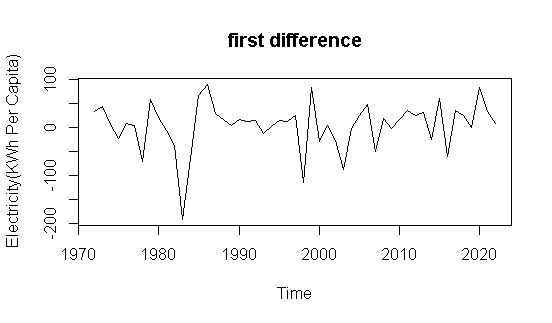
\includegraphics[width=0.9\linewidth]{images/image2}
			\end{center}
		
			\caption{First difference plot}
		\end{figure}

	\end{frame}

	\begin{frame}{Stationarity Testing For Differenced Data}
		\begin{block}{Augmented Dickey-Fuller Test}
			data: diff1 Dickey-Fuller = -4.8579, Lag order = 3, p-value = 0.01 alternative hypothesis: stationary \vspace{5pt}
		\end{block}
		
		\begin{alertblock}{KPSS Test for Level Stationarity}
			data: diff1 KPSS Level = 0.14346, Truncation lag parameter = 3, p-value = 0.1 \vspace{5pt}
		\end{alertblock}
		
		\begin{exampleblock}{Phillips-Perron Unit Root Test}
			data: diff1 Dickey-Fuller Z(alpha) = -43.687, Truncation lag parameter = 3, p-value = 0.01 alternative hypothesis: stationary.
		\end{exampleblock}
	\end{frame}
	
\end{document}